\documentclass[twocolumn,10pt]{article}

\usepackage[english]{babel}
\usepackage[utf8]{inputenc}
\usepackage[T1]{fontenc}
\usepackage{listings}
\usepackage{graphicx}
\usepackage{comment}
\usepackage{amsmath}
\usepackage{hyperref}



\title{Assessed Coursework 2 Report\linebreak Distributed Algorithms and Systems}

\author{Willian de Oliveira Barreiros Junior\\
Matric Number: 2105514\\
 guns945@gmail.com\\}

\begin{document}
\maketitle

\section{Introduction}
This report regards the implementation details of a bidding system. The system consists of two java programs, a central server and a client. The system was conceived to ensure, first, data concistency, second, escalability, and finally, efficiency with multiple clients.

This report is divided into four parts, a thoroughly explanation on the server implementation and the structures used by it, the details on the client implementation, the tests performed, and finally, the conclusion, containing some final observations on the final implementation, the tests and possible future improvements.

The source code from this coursework can also be found at
\url{https://github.com/WillianJunior/DASProject1}

\section{Server Implementation}


\begin{equation}\label{eq:sceneCost}
cost[i] = duration[i]\times\sum_{j=0}^{actors}timetable[j][i]\times cost[j]
\end{equation}

\begin{figure}[h]
\centering
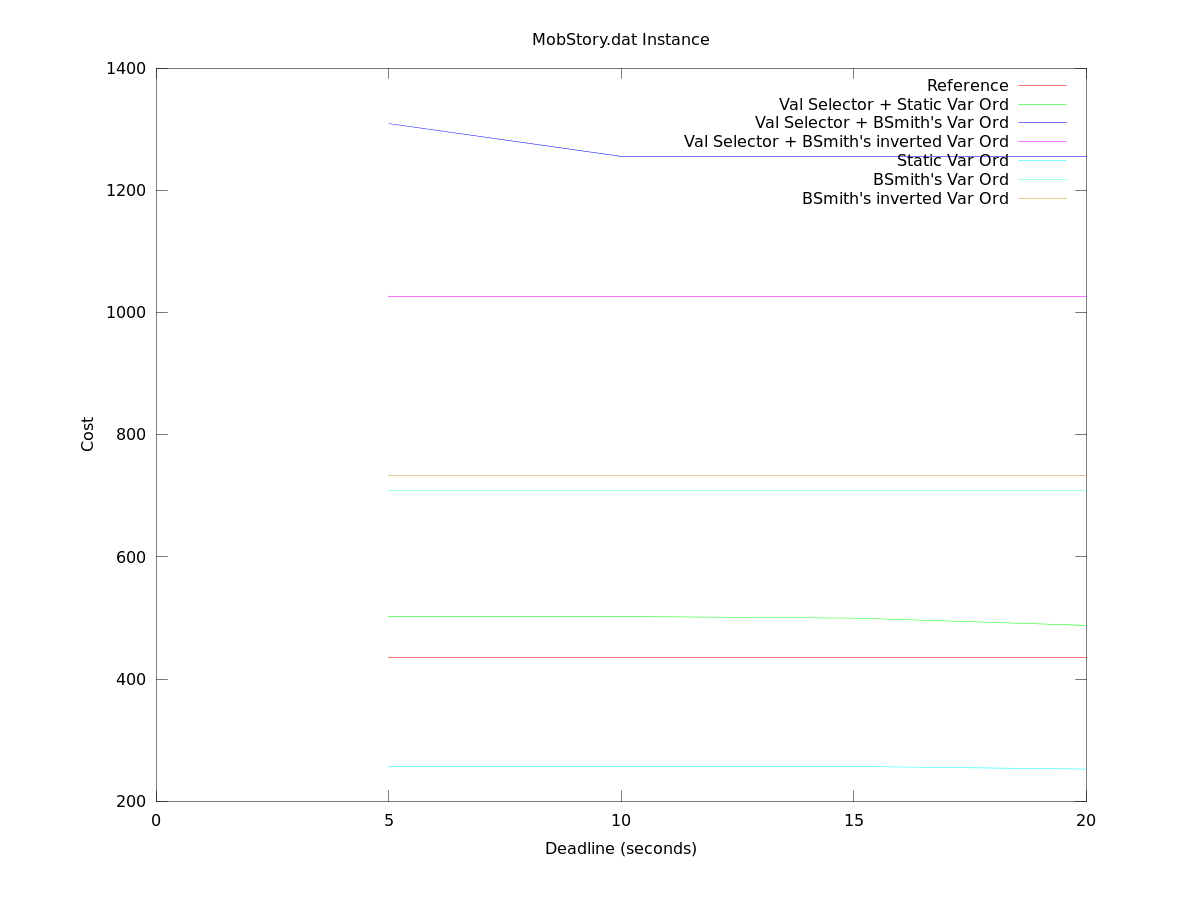
\includegraphics[scale=0.18]{mobs.png}
\caption{Comparison of the heuristics using the MobStory.dat file}
\label{fig:mobs}
\end{figure}

\end{document}
